\chapter{Технологический раздел}

В этом разделе будет обоснован выбор языка программирования и среды разработки, рассмотрена диаграмма основных классов и разобран интерфейс, предлагаемый пользователю.

\section{Выбор языка программирования и среды разработки}
При разработке программного продукта был использован язык программирования Python (версия 3.8.10) \cite{pythonlang}.

Данный выбор был сделан по следующим причинам.
\begin{enumerate}
	\item Опыт работы с рассматриваемым языком.
	\item Поддержка объектно-ориентированного подхода к программированию.
	\item Большое количество литературы, связанной с ЯП Python.
\end{enumerate}

В качестве среды разработки были использованы PyCharm \cite{pycharm} и Visual Studio Code \cite{vcode}, поскольку они бесплатны для студентов, удобны в процессе разработки и ранее активно использовались.

Время работы приложения измерялось при помощью функции \newline $process\_time()$ из библиотеки $time$ \cite{pythonlangtime}. Для создания GUI (Graphical User Interface) был использован модуль $PyQt5$ \cite{pyqt5}.

\section{Подключение к базам данных}

Для подключения к той или иной базе данных нужно иметь информацию о ней: адрес подключения, используемый драйвер,тип СУБД, логин и пароль пользователя.

Для ввода данной информации в интерфейсе предоставлены специальные поля. На рисунке \ref{img:interf_con} показаны данные поля.

\begin{figure}[h!]
	\begin{center}
		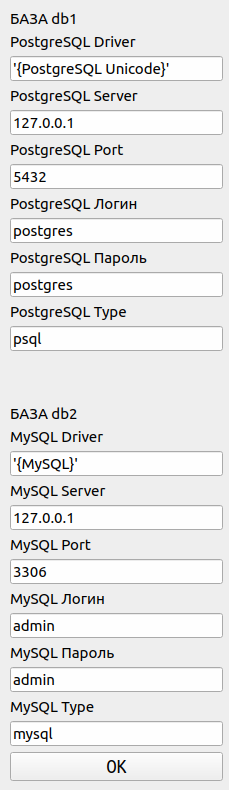
\includegraphics[scale=0.75]{./inc/img/interf_con}
		\caption{Поля для подключения к СУБД}
		\label{img:interf_con}
	\end{center}
\end{figure}

В данном примере $db1$ и $db2$ уникальное имя СУБД, которое будет использовать пользователь, чтобы указать какая именно БД используется в данном запросе. $PostgreSQL Driver$ и $MySQL Driver$ -- названия драйверов, данные поля уже заполнены по умолчанию. $PostgreSQL Server$ и \newline $MySQL Server$ -- адреса баз данных, поля заполнены для подключению к локальным базам данных. $PostgreSQL Type$ и $MySQL Type$ -- типы СУБД.

\section{Используемая база данных}

На рисунке \ref{img:er_db} представлена ER-диаграмма базы данных, которая использовалась для проверки работы приложения.

Данная база данных была разделена по различным СУБД, как показано на рисунке \ref{img:er_db}, а также для проверки работы данная база данных была расположена в одной СУБД (PostgreSQL).

\begin{figure}[h!]
	\begin{center}
		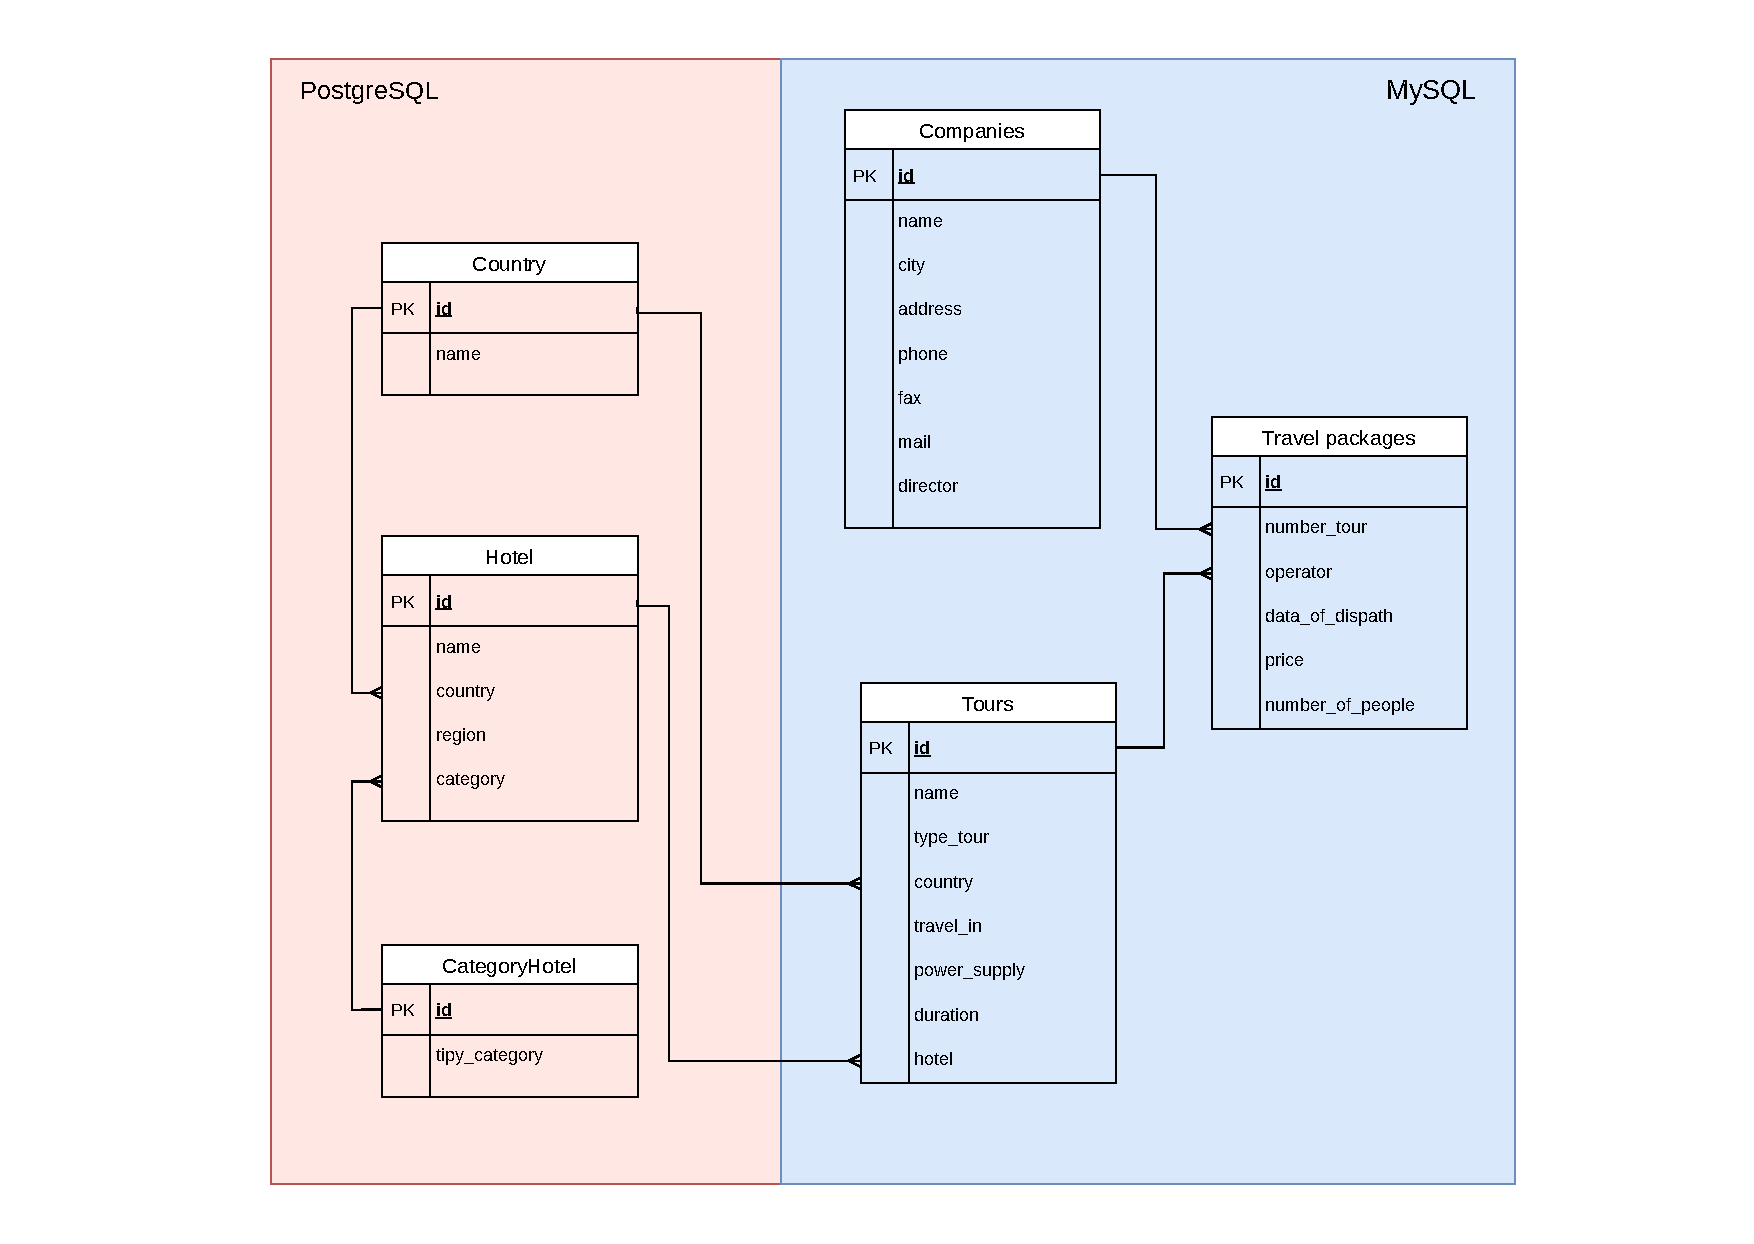
\includegraphics[scale=0.7]{./inc/img/er_db.pdf}
		\caption{Диаграмма БД}
		\label{img:er_db}
	\end{center}
\end{figure}

\subsection{Создание таблиц}

В соответствие со схемой выше было создано 3 таблицы в PostgreSQL СУБД и 3 таблицы в СУБД MySQL.

Создание некоторых из них приведено, а именно hotels в PostgreSQL и tours в MySQL представлено в листинге \ref{lst:create_db}.

\begin{lstlisting}[label=lst:create_db,caption=Создание некоторых таблиц]
-- PostgreSQL
CREATE TABLE IF NOT EXISTS Hotels(
	HotelId INT GENERATED ALWAYS AS IDENTITY PRIMARY KEY,
	NameHotel VARCHAR(100) NOT NULL, -- имя
	CountryId INT, -- номер страны
	Region VARCHAR(100) NOT NULL, -- название региона
	CategoryId -- номер категории
);

-- MySQL
CREATE TABLE sys.Tours(
	TourId INT  PRIMARY KEY,
	NameTour VARCHAR(100) NOT NULL, -- имя тура
	TypeTour VARCHAR(100) NOT NULL, -- тип тура
	CountryId INT, -- номер страны
	TravelOnOff INT, -- дорога входит или нет
	PowerSupply INT, -- питание сколько раз
	Duration INT, -- длительность
	HotelId INT -- номер отеля
);

\end{lstlisting}

Следует отметить, что в PostgreSQL используется автогенерация первичного ключа (в таблице hotels это hotelid). 

\subsection{Наполнение таблиц}

Таблицы заполняются сгенерированными данными с помощью библиотеки Faker \cite{faker}.

Полученные данные записываются в файл, из которого далее будут подгружаться данные. На листинге \ref{lst:gener_db} приведены функции генерации данных для таблицы отелей (hotels) и туров (tours). Другие таблицы заполняются аналогично.

\begin{lstlisting}[label=lst:gener_db,caption=Генерация данных для таблиц]
# Функция генерации данных для таблицы Отелей
cat_hotel = [1, 2, 3, 4, 5]
def generate_hotel():
	faker = Faker()
	f = open('hotel.csv', 'w')
	for i in range(MAX_N):
		country = randint(1, 239)
		line = "{0};{1};{2};{3}\n".format(
			faker.name(),
			country,
			faker.country() + "Region" + str(choice(cat_hotel)),
			choice(cat_hotel)
		)
		f.write(line)
	f.close()
	
# Функция генерации данных для таблицы Туров
on_off = [0, 1]
eat = [1, 2, 3]
t_tour = ["beach", "excursion", "sports", "quiet", "mobile"]
def generate_tours():
	faker = Faker()
	f = open('tour.csv', 'w')
	for i in range(MAX_N):
		week = randint(1, 6)
		hotel = randint(1, 999)
		country = randint(1, 239)
		line = "{0};{1};{2};{3};{4};{5};{6}\n".format(
			faker.name(),
			choice(t_tour),
			country,
			choice(on_off),
			choice(eat),
			week,
			hotel,
		)
		f.write(line)
	f.close()

\end{lstlisting}

\section{Структура программы}

При написании программы используется язык Python, что дает возможность использовать его со стороны объектно-ориентированного подхода.

Условно классы в программе можно разделить на следующие группы.
\begin{enumerate}
	\item Semantic\_analyzer -- класс, описывающий работу семантического анализатора.
	\item BaseDialect, MySQL, PostgreSQL -- группа классов, описывающих диалекты MySQL и PostgreSQL.
	\item BaseToken, EndToken, IntToken, IdentifierToken, StringToken, FloatToken, SymbolToken, KeywordToken,  DateToken -- группа классов, описывающих все возможные токены.
	\item Sintactic\_analyzer, SQLParser -- группа классов, описывающих синтаксический анализатор.
	\item Lexer\_analyzer -- группа классов, описывающих лексический анализатор.
	\item BaseJoin, InnerJoin -- группа классов, описывающих работу Inner Join.
\end{enumerate}

На рисунке \ref{img:uml} представлена структура и состав классов.

\begin{figure}[h!]
	\begin{center}
		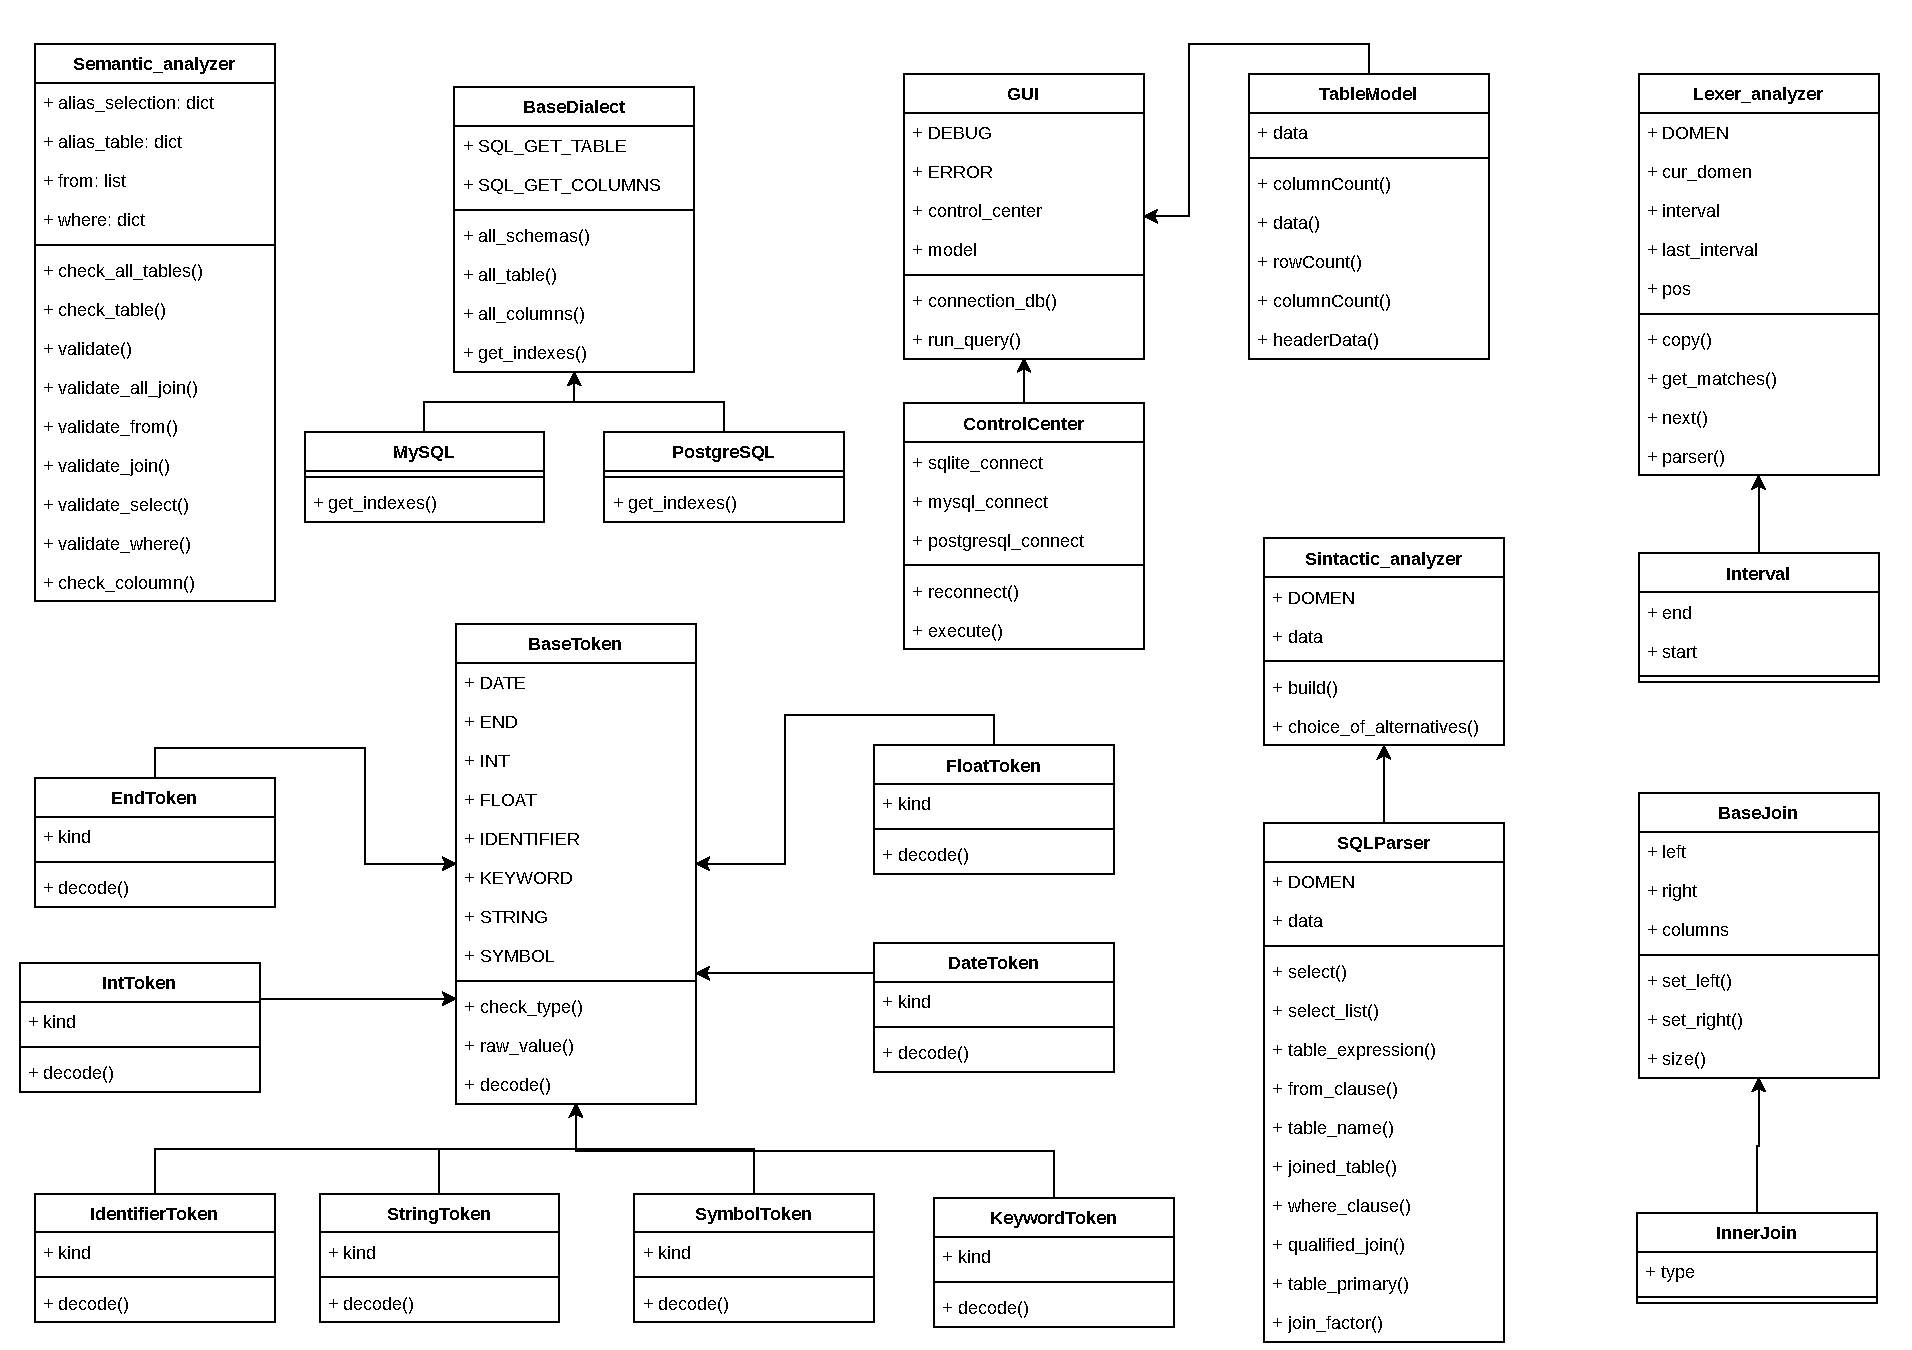
\includegraphics[scale=0.5]{./inc/img/uml}
		\caption{Структура программы}
		\label{img:uml}
	\end{center}
\end{figure}
\newpage

\section{Интерфейс}

На рисунке \ref{img:interf} представлен интерфейс программы.

\begin{figure}[h!]
	\begin{center}
		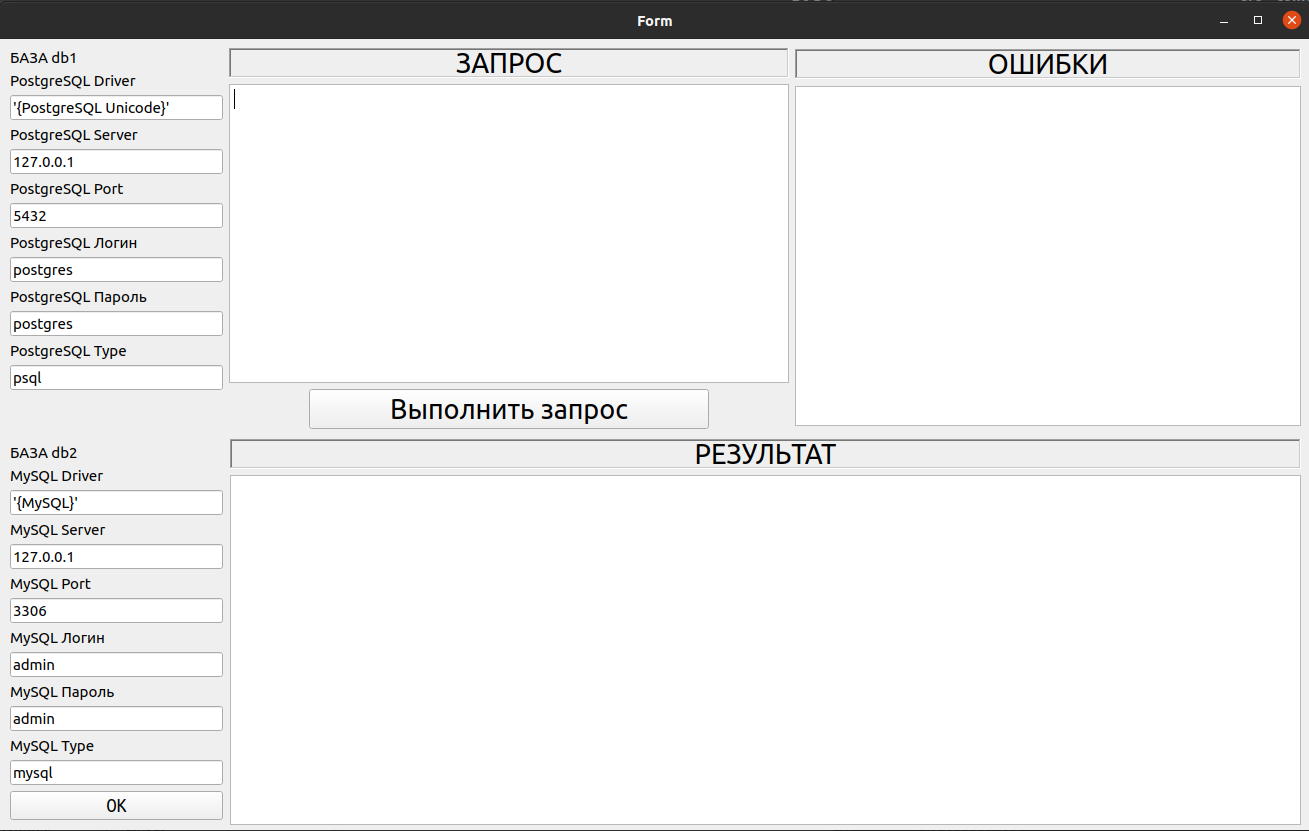
\includegraphics[scale=0.5]{./inc/img/interf}
		\caption{Интерфейс приложения}
		\label{img:interf}
	\end{center}
\end{figure}

Функции предоставленных кнопок следующие:
\begin{itemize}
	\item поле <<ЗАПРОС>> -- поле для ввода SQL запроса;
	\item поле <<ОШИБКИ>> -- если в результате выполнения запроса возникают ошибки, то эти ошибки пишутся в данное поле на экране;
	\item поле <<РЕЗУЛЬТАТ>> -- поля для вывода результата;
	\item кнопка <<ОК>> -- выполняется подключение к базам данных;
	\item кнопка <<Выполнить запрос>> -- выполняется запрос, записанный в поле <<ЗАПРОС>>
\end{itemize}


\section{Результаты работы программного обеспечения}

На рисунке \ref{img:work1} представлен результат запроса \ref{lst:mysql}, выполненного непос\-редственно напрямую в СУБД MySQL.

На рисунке \ref{img:work1_1} представлен результат этого же запроса (запрос \ref{lst:mysql}), выполненного с помощью приложения.

\begin{lstlisting}[label=lst:mysql,caption=Запрос в MySQL]
select *
from puplic.sys.Tours
\end{lstlisting}

\begin{figure}[h!]
	\begin{center}
		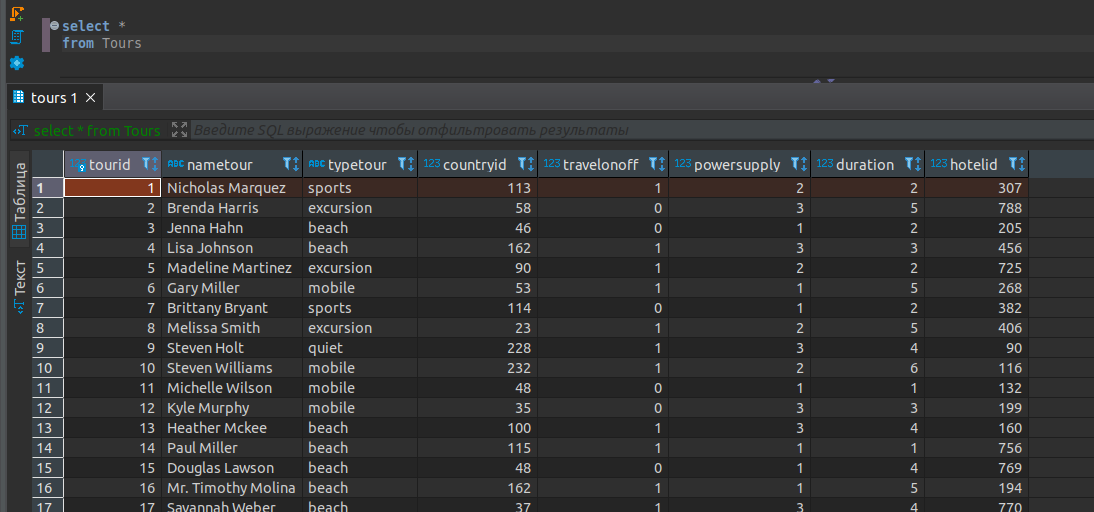
\includegraphics[scale=0.55]{./inc/img/mysql1}
		\caption{Результат запроса в MySQL}
		\label{img:work1}
	\end{center}
\end{figure}

\begin{figure}[h!]
	\begin{center}
		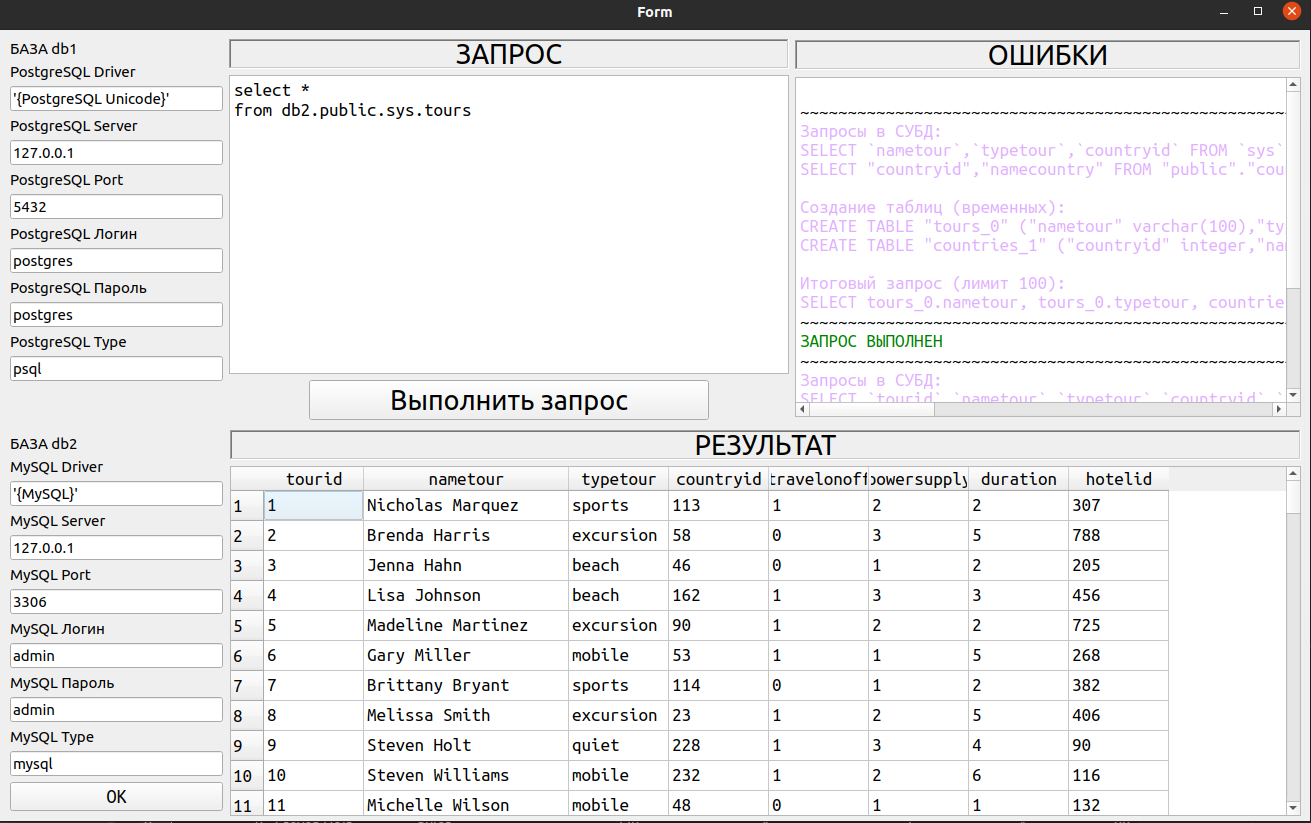
\includegraphics[scale=0.4]{./inc/img/mysql1_1}
		\caption{Результат запроса, выполненного через приложение}
		\label{img:work1_1}
	\end{center}
\end{figure}

\newpage

На рисунке \ref{img:work2} представлен результат запроса \ref{lst:postgres}, выполненного непос\-редственно напрямую в СУБД PostgreSQL.

На рисунке \ref{img:work2_1} представлен результат этого же запроса (запрос \ref{lst:postgres}), выполненного с помощью приложения.

\begin{lstlisting}[label=lst:postgres,caption=Запрос в PostgreSQL]
select *
from postgres.public.hotels 
\end{lstlisting}

\begin{figure}[h!]
	\begin{center}
		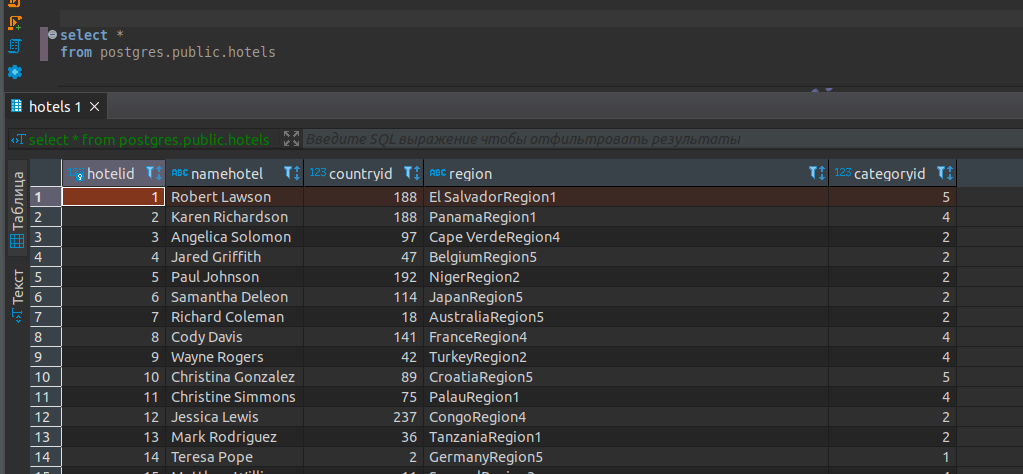
\includegraphics[scale=0.6]{./inc/img/postgres1}
		\caption{Результат запроса в PostgreSQL}
		\label{img:work2}
	\end{center}
\end{figure}

\begin{figure}[h!]
	\begin{center}
		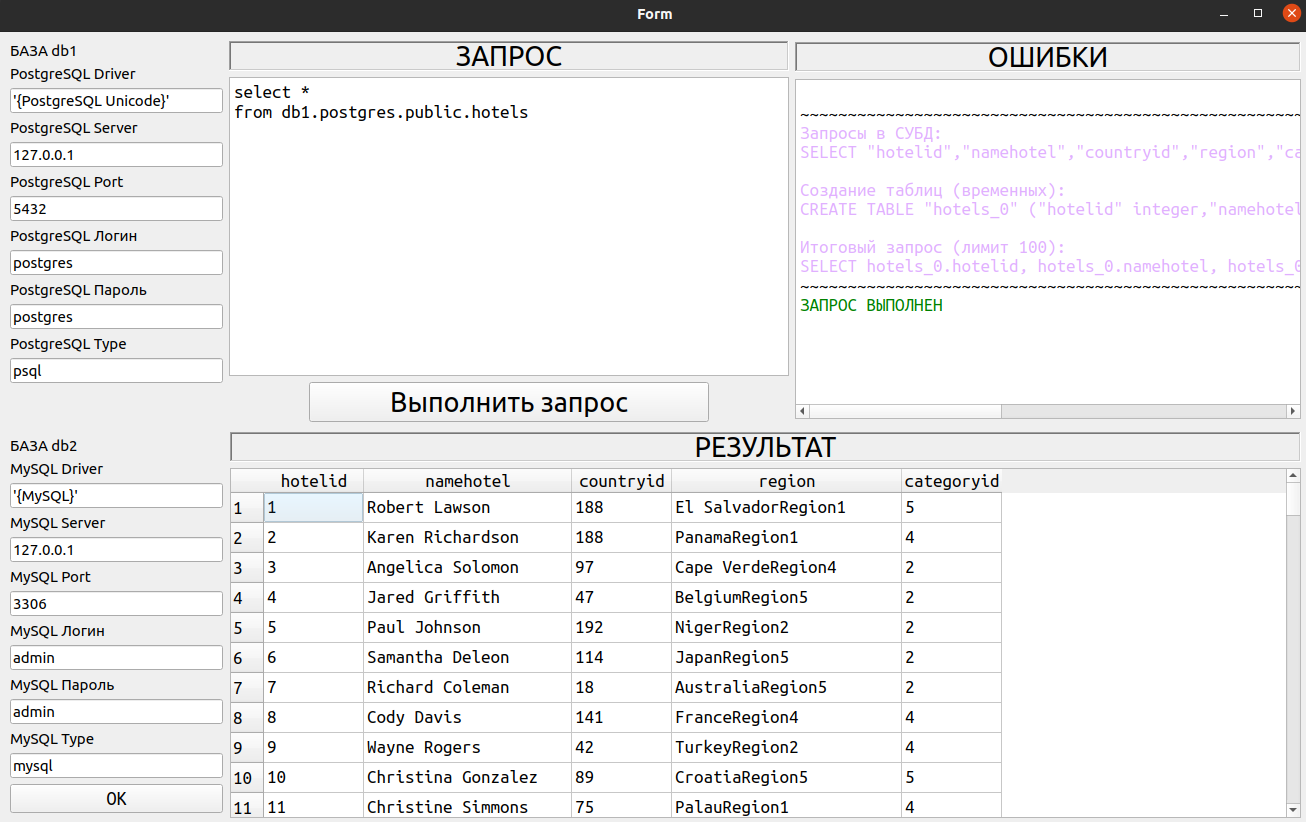
\includegraphics[scale=0.4]{./inc/img/postgres1_1}
		\caption{Результат запроса в PostgreSQL}
		\label{img:work2_1}
	\end{center}
\end{figure}

\newpage

\section{Тестирование}

На рисунке \ref{img:test1} представлен результат выполнения запроса \ref{lst:test1}. 

Здесь и далее: в правой части рисунка результат, полученный приложением, в левой -- результат, в случае, когда все таблицы расположены в одной СУБД (в данном случае PostgreSQL). 

Данный запрос направлен на тестирование оператора JOIN двух таблиц из разных СУБД.

\begin{figure}[h!]
	\begin{center}
		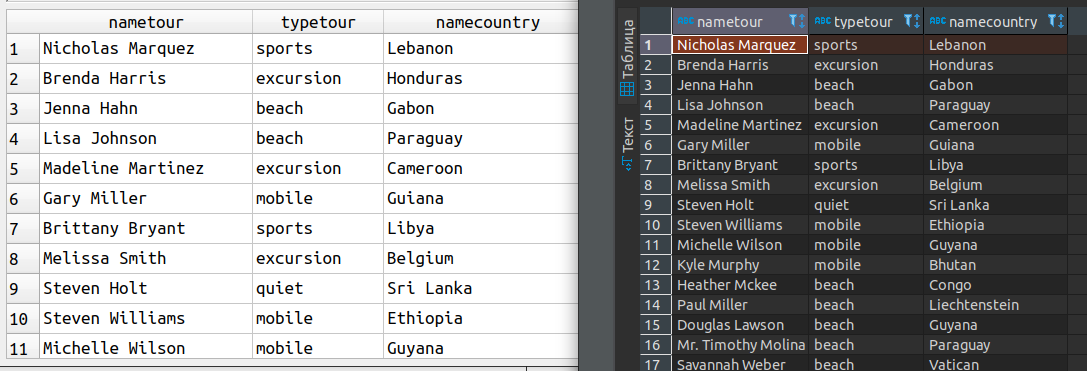
\includegraphics[scale=0.6]{./inc/img/test1}
		\caption{Результат запроса \ref{lst:test1}}
		\label{img:test1}
	\end{center}
\end{figure}


\begin{lstlisting}[label=lst:test1,caption=Запрос в PostgreSQL и приожения]
-- Запрос в СУБД PostgreSQL
select t.NameTour, t.TypeTour, c.NameCountry
from Tours as t join Countries as c on t.CountryId = c.CountryId

-- Запрос в приложении
select t.nametour, t.typetour, c.namecountry
from db2.public.sys.tours as t join db1.postgres.public.countries as c on t.countryid = c.countryid
\end{lstlisting}



На рисунке \ref{img:test2} представлен результат выполнения запроса \ref{lst:test2}. 

Данный запрос направлен на тестирование оператора WHERE для выборки из таблицы, расположенной в MySQL.
\clearpage
\begin{figure}[h!]
	\begin{center}
		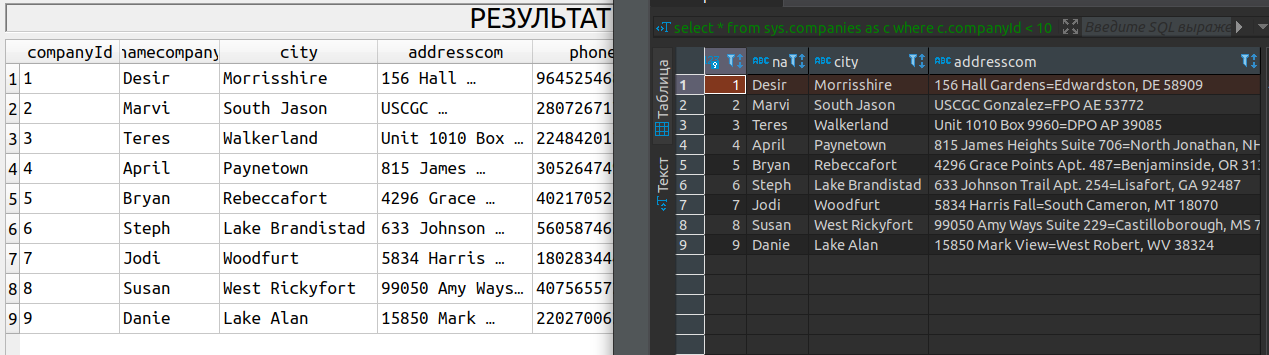
\includegraphics[scale=0.5]{./inc/img/test2}
		\caption{Результат запроса \ref{lst:test2}}
		\label{img:test2}
	\end{center}
\end{figure}

\begin{lstlisting}[label=lst:test2,caption=Запрос в MySQL и приложение]
-- Запрос в СУБД MySQL
select *
from sys.companies as c
where c.companyId  < 10

-- Запрос в приложении
select *
from db2.public.sys.companies as c
where c.companyId  < 10
\end{lstlisting}





На рисунке \ref{img:test3} представлен результат выполнения запроса \ref{lst:test3}. 

Данный запрос направлен на тестирование оператора WHERE для выборки из таблицы, расположенной в PostgreSQL.

\begin{figure}[h!]
	\begin{center}
		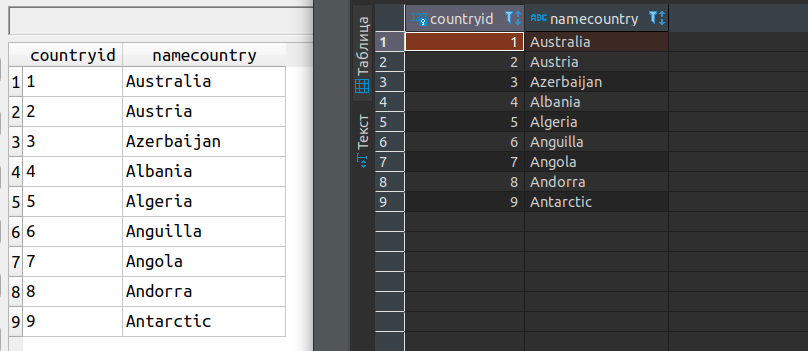
\includegraphics[scale=0.6]{./inc/img/test3}
		\caption{Результат запроса \ref{lst:test3}}
		\label{img:test3}
	\end{center}
\end{figure}

\begin{lstlisting}[label=lst:test3,caption=Запрос в PostgreSQL и приложение]
-- Запрос в СУБД PostgreSQL
select *
from postgres.public.countries c 
where c.countryid < 10

-- Запрос в приложении
select *
from db1.postres.public.countries as c
where c.countryid  < 10
\end{lstlisting}




На рисунке \ref{img:test4} представлен результат выполнения запроса \ref{lst:test4}. 

Данный запрос направлен на тестирование операторов JOIN и WHERE одновременно.

\begin{figure}[h!]
	\begin{center}
		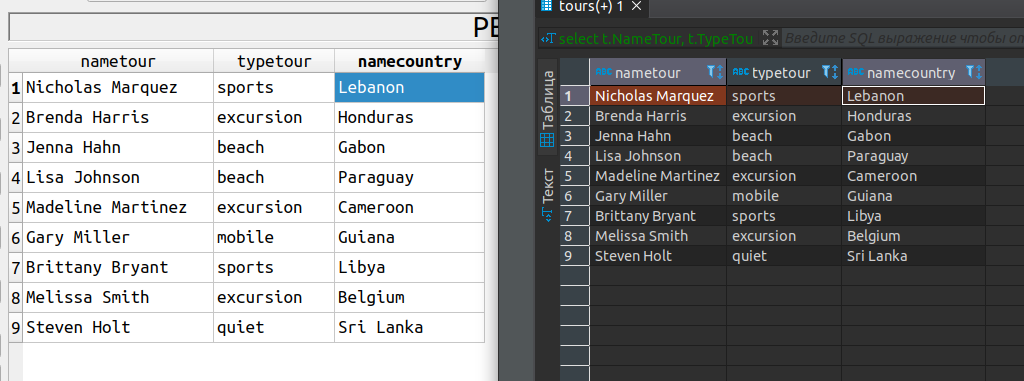
\includegraphics[scale=0.6]{./inc/img/test4}
		\caption{Результат запроса \ref{lst:test4}}
		\label{img:test4}
	\end{center}
\end{figure}


\begin{lstlisting}[label=lst:test4,caption=Запрос в PostgreSQL и приложение]
-- Запрос в СУБД PostgreSQL
select t.NameTour, t.TypeTour, c.NameCountry
from Tours as t join Countries as c on t.CountryId = c.CountryId
where t.tourid < 10

-- Запрос в приложении
select t.nametour, t.typetour, c.namecountry
from db2.public.sys.tours as t join db1.postgres.public.countries as c on t.countryid = c.countryid
where t.tourid < 10
\end{lstlisting}





\section{Вывод}

В этом разделе был выбран язык программирования и среда разработки, рассмотрена UML-диаграмма основных классов, подробно разобран интерфейс приложения, приведены результаты тестирования, а также протестированного разработанное приложение.

В курсовой работе рассматривались лишь два оператора WHERE и JOIN. Исследование и разработка в этом направлении могут быть продолжены до реализации полного функционала работы СУБД.